\section{Информационный менеджмент}

	\subsection{Ресурсная матрица проекта}

	Целью создания данной ИС служит автоматизация процесса проверки работ на плагиат. Оценку эффективности внедрения ИС можно проводить по нескольким показателям, в том числе и по сокращению временных затрат. Для этого необходимо построить ресурсные матрицы для процесса до и после автоматизации, и на их основе рассчитать эффективность от внедрения.

		\subsubsection{Ресурсная матрица процесса до автоматизации}	

			Процесс проверки работы на плагиат до автоматизации состоял из следующих операций:
			\begin{itemize}
				\item загрузка работы студента на локальную машину сотрудника;
				\item нахождение работ в системе <<Moodle>> для сравнения;
				\item ручная сверка новой работы с другими работами.
			\end{itemize}

			В таблице \ref{tab:resources_before} представлены ресурсы, которые используются в процессе до автоматизации.

			\begin{table}[h]
				\centering
				\caption{Ресурсная матрица процесса до автоматизации}
				\label{tab:resources_before}				
				\begin{tabular}{|l|l|l|}
				\hline
					\multicolumn{1}{|c|}{$Р_{Сотр}$} 				&
					\multicolumn{1}{ c|}{$Р_{\text{Сотр-Moodle}}$} 	&
					\multicolumn{1}{ c|}{$Р_{\text{Сотр-Local}}$} 	\\ \hline
					\multicolumn{1}{|c|}{$Р_{\text{Сотр-Moodle}}$} 	&
					\multicolumn{1}{ c|}{$Р_{\text{Moodle}}$} 		&
					\multicolumn{1}{ c|}{$-$} 						\\ \hline
					\multicolumn{1}{|c|}{$Р_{\text{Сотр-Local}}$} 	&
					\multicolumn{1}{ c|}{$-$} 						&
					\multicolumn{1}{ c|}{$Р_{\text{Local}}$}			\\ \hline                           
				\end{tabular}
			\end{table}			

			\newpage
			В таблице \ref{tab:resources_ref_before} приведено описание ресурсов из таблицы \ref{tab:resources_before}.

			\begin{table}[h]
				\small
				\centering
				\caption{Компоненты ресурсной матрицы до автоматизации}
				\label{tab:resources_ref_before}				
				\begin{tabular}{|l|l|}				
				\hline
					\multicolumn{1}{|c|}{Ресурс} 										&
					\multicolumn{1}{ c|}{Описание} 										\\ \hline
					$Р_{\text{Сотр}}$													&
					Сотрудник учебного заведения (25\,000 руб./мес. или 142 руб./час) 	\\ \hline
					$Р_{\text{Moodle}}$													&
					Рабочая станция с установленной ИС <<Moodle>> (30\,000 руб.) 		\\ \hline
					$Р_{\text{Local}}$													&
					Рабочая станция сотрудника (25\,000 руб.)							\\ \hline
					$Р_{\text{Сотр-Moodle}}$											&
					Взаимодействие сотрудника с ИС <<Moodle>> (180 мин./день)			\\ \hline
					$Р_{\text{Сотр-Local}}$												&
					Рабочий процесс сотрудника на локальном ПК (30 мин./день)			\\ \hline
				\end{tabular}
			\end{table}			

			В качестве значений для ресурсов $Р_{\text{Moodle}}$ и $Р_{\text{Local}}$ рассчитывается амортизация этого оборудования за месяц - 500 руб. и 415 руб. соответственно.

			Значение для ресурса $Р_{\text{Сотр-Moodle}}$ рассчитывается как 180 * 3 * 4 = 21 час/мес., так как в среднем сотрудник проверяет работы 3-х групп за неделю. Соответственно, значение для $Р_{\text{Сотр-Local}}$ определяется как 30 * 3 * 4 = 6 часов/мес.			

			\begin{table}[h]
				\centering
				\caption{Временная ресурсная матрица до автоматизации}
				\label{tab:time_resources_before}				
				\begin{tabular}{|l|l|l|}
				\hline
					\multicolumn{1}{|c|}{25\,000} 	&
					\multicolumn{1}{ c|}{2\,982 } 	&
					\multicolumn{1}{ c|}{852} 		\\ \hline
					\multicolumn{1}{|c|}{2\,982} 	&
					\multicolumn{1}{ c|}{500} 		&
					\multicolumn{1}{ c|}{0} 			\\ \hline
					\multicolumn{1}{|c|}{852} 		&
					\multicolumn{1}{ c|}{0} 			&
					\multicolumn{1}{ c|}{415}		\\ \hline                           
				\end{tabular}
			\end{table}	

			\begin{table}[h]
				\centering
				\caption{Нормированная временная ресурсная матрица до автоматизации}
				\label{tab:normalization_time_resources_before}				
				\begin{tabular}{|l|l|l|}
				\hline
					\multicolumn{1}{|c|}{1,000} 	&
					\multicolumn{1}{ c|}{0,119} 		&
					\multicolumn{1}{ c|}{0,034} 		\\ \hline
					\multicolumn{1}{|c|}{0,119} 	&
					\multicolumn{1}{ c|}{0,020} 		&
					\multicolumn{1}{ c|}{0,000} 		\\ \hline
					\multicolumn{1}{|c|}{0,034} 	&
					\multicolumn{1}{ c|}{0,000} 		&
					\multicolumn{1}{ c|}{0,016}		\\ \hline                           
				\end{tabular}
			\end{table}								

			В таблице \ref{tab:time_resources_before} представлены сводные значения по ресурсам, а в таблице \ref{tab:normalization_time_resources_before}  приведены значения после нормировкии относительно ресурса $Р_{\text{Сотр}}$.

			\newpage
			В таблице \ref{tab:resource_costs_before} приведены коэффициенты использования каждого ресурса по операциям.

			\begin{table}[h]
				\small
				\centering
				\caption{Затраты ресурсов на выполнение операций до автоматизации}
				\label{tab:resource_costs_before}				
				\begin{tabular}{|l|l|l|l|}				
				\hline
					\multicolumn{1}{|c|}{Ресурсы} 										&
					\multicolumn{1}{ c|}{Операция 1} 									&
					\multicolumn{1}{ c|}{Операция 2} 									&
					\multicolumn{1}{ c|}{Операция 3} 									\\ \hline
					$Р_{\text{Сотр}}$													&
					\multicolumn{1}{ c|}{0,05}											&
					\multicolumn{1}{ c|}{0,10}																&
					\multicolumn{1}{ c|}{0,85}																\\ \hline
					$Р_{\text{Moodle}}$													&
					\multicolumn{1}{ c|}{0,10}																&
					\multicolumn{1}{ c|}{0,50}															&
					\multicolumn{1}{ c|}{0,40}																\\ \hline
					$Р_{\text{Local}}$													&
					\multicolumn{1}{ c|}{0,20}															&
					\multicolumn{1}{ c|}{0,00}																&
					\multicolumn{1}{ c|}{0,80}																\\ \hline
					$Р_{\text{Сотр-Moodle}}$											&
					\multicolumn{1}{ c|}{0,10}																&
					\multicolumn{1}{ c|}{0,80}																&
					\multicolumn{1}{ c|}{0,10}																\\ \hline
					$Р_{\text{Сотр-Local}}$												&
					\multicolumn{1}{ c|}{0,20}																&
					\multicolumn{1}{ c|}{0,00}																&
					\multicolumn{1}{ c|}{0,80}																\\ \hline
				\end{tabular}
			\end{table}

			Для оценки качества работы ИС и объема выполненных ею работ необходимо определить некоторые количественные меры, что позволит корректно вычислять соответствующие функционалы, например взвешенную сумму $Ф_к$ затраченных на выполнение k-ого технологического процесса ресурсов вида \ref{eq:functional_before}:
			\begin{equation}\label{eq:functional_before}
				Ф_к = (\sum_{r=1}^{m_k} f_r Р_r)_к,				
			\end{equation}
			\begin{ESKDexplanation}
				\item[где ] $r$ 		--- индекс суммирования затрат составляющих ресурсов по k-ому технологическому маршруту;
				\item $m_k$ --- число операций k-ого технологического процесса;
				\item $f_r$ --- весовой коэффициент r-ого компонента ресурса.
			\end{ESKDexplanation}

			Расчет эффективности для описанного процесса:

			$Ф_1 = 0,05 * 1,000 + 0,10 * 0,020 + 0,20 * 0,016 + 0,10 * 0,119 + 0,20 * 0,034 = 0,074;$

			$Ф_2 = 0,10 * 1,000 + 0,50 * 0,020 + 0,80 * 0,119 = 0,205;$

			$Ф_3 = 0,85 * 1,000 + 0,40 * 0,020 + 0,80 * 0,016 + 0,10 * 0,119 + 0,80 * 0,034 = 0,910;$

			$Ф = 1,189.$

		\subsubsection{Ресурсная матрица процесса после автоматизации}	

			Процесс проверки работы на плагиат после автоматизации состоит из следующих операций:
			\begin{itemize}
				\item обработка запроса системой проверки на плагиат;
				\item просмотр результата проверки работ на плагиат;				
				\item анализ результата проверки.
			\end{itemize}

			В таблице \ref{tab:resources_after} представлены ресурсы, которые используются в процессе после автоматизации.

			\begin{table}[h]
				\centering
				\caption{Ресурсная матрица процесса после автоматизации}
				\label{tab:resources_after}				
				\begin{tabular}{|l|l|l|}
				\hline
					\multicolumn{1}{|c|}{$Р_{Сотр}$} 				&
					\multicolumn{1}{ c|}{$Р_{\text{Сотр-Moodle}}$} 	&
					\multicolumn{1}{ c|}{$-$} 	\\ \hline
					\multicolumn{1}{|c|}{$Р_{\text{Сотр-Moodle}}$} 	&
					\multicolumn{1}{ c|}{$Р_{\text{Moodle}}$} 		&
					\multicolumn{1}{ c|}{$-$} 						\\ \hline
					\multicolumn{1}{|c|}{$-$} 	&
					\multicolumn{1}{ c|}{$-$} 						&
					\multicolumn{1}{ c|}{$Р_{\text{Шерлок}}$}			\\ \hline                           
				\end{tabular}
			\end{table}					
			
			В таблице \ref{tab:resources_ref_after} приведено описание ресурсов из матрицы.

			\begin{table}[h]
				\small
				\centering
				\caption{Компоненты ресурсной матрицы после автоматизации}
				\label{tab:resources_ref_after}				
				\begin{tabular}{|l|l|}				
				\hline
					\multicolumn{1}{|c|}{Ресурс} 										&
					\multicolumn{1}{ c|}{Описание} 										\\ \hline
					$Р_{\text{Сотр}}$													&
					Сотрудник учебного заведения (25\,000 руб./мес. или 142 руб./час) 	\\ \hline
					$Р_{\text{Moodle}}$													&
					Рабочая станция с установленной ИС <<Moodle>> (30\,000 руб.) 		\\ \hline
					$Р_{\text{Шерлок}}$													&
					Рабочая станция с ИС <<Шерлок>> (25\,000,00 руб.)					\\ \hline
					$Р_{\text{Сотр-Moodle}}$											&
					Взаимодействие сотрудника с ИС <<Moodle>> (10 мин./день)			\\ \hline
				\end{tabular}
			\end{table}		

			В качестве значений для ресурсов $Р_{\text{Moodle}}$ и $Р_{\text{Шерлок}}$ рассчитывается амортизация этого оборудования за месяц - 500,00 руб. и 415,00 руб. соответственно.

			Значение для ресурса $Р_{\text{Сотр-Moodle}}$ рассчитывается как 20 * 3 * 4 = 2 часа/мес., так как в среднем сотрудник проверяет работы 3-х групп за неделю.

			\newpage
			В таблице \ref{tab:time_resources_after} представленны сводные значения по ресурсам, а в таблице \ref{tab:normalization_time_resources_after}  приведены значения после нормировкии относительно ресурса $Р_{\text{Сотр}}$.

			\begin{table}[h]
				\centering
				\caption{Временная ресурсная матрица после автоматизации}
				\label{tab:time_resources_after}				
				\begin{tabular}{|l|l|l|}
				\hline
					\multicolumn{1}{|c|}{25\,000} 	&
					\multicolumn{1}{ c|}{284 } 	&
					\multicolumn{1}{ c|}{0} 		\\ \hline
					\multicolumn{1}{|c|}{284} 	&
					\multicolumn{1}{ c|}{500} 		&
					\multicolumn{1}{ c|}{0} 			\\ \hline
					\multicolumn{1}{|c|}{0} 		&
					\multicolumn{1}{ c|}{0} 			&
					\multicolumn{1}{ c|}{415}		\\ \hline                           
				\end{tabular}
			\end{table}	

			\begin{table}[h]
				\centering
				\caption{Нормированная временная ресурсная матрица после автоматизации}
				\label{tab:normalization_time_resources_after}				
				\begin{tabular}{|l|l|l|}
				\hline
					\multicolumn{1}{|c|}{1,000} 	&
					\multicolumn{1}{ c|}{0,011} 		&
					\multicolumn{1}{ c|}{0,000} 		\\ \hline
					\multicolumn{1}{|c|}{0,011} 	&
					\multicolumn{1}{ c|}{0,020} 		&
					\multicolumn{1}{ c|}{0,000} 		\\ \hline
					\multicolumn{1}{|c|}{0,000} 	&
					\multicolumn{1}{ c|}{0,000} 		&
					\multicolumn{1}{ c|}{0,016}		\\ \hline                           
				\end{tabular}
			\end{table}				

			В таблице \ref{tab:resource_costs_after} приведены коэффициенты использования каждого ресурса по операциям.

			\begin{table}[h]
				\small
				\centering
				\caption{Затраты ресурсов на выполнение операций после автоматизации}
				\label{tab:resource_costs_after}				
				\begin{tabular}{|l|l|l|l|}				
				\hline
					\multicolumn{1}{|c|}{Ресурсы} 										&
					\multicolumn{1}{ c|}{Операция 1} 									&
					\multicolumn{1}{ c|}{Операция 2} 									&
					\multicolumn{1}{ c|}{Операция 3} 									\\ \hline
					$Р_{\text{Сотр}}$													&
					\multicolumn{1}{ c|}{0,00}																&
					\multicolumn{1}{ c|}{0,30}																&
					\multicolumn{1}{ c|}{0,70}																\\ \hline
					$Р_{\text{Moodle}}$													&
					\multicolumn{1}{ c|}{0,20}																&
					\multicolumn{1}{ c|}{0,70}																&
					\multicolumn{1}{ c|}{0,10}																\\ \hline
					$Р_{\text{Шерлок}}$													&
					\multicolumn{1}{ c|}{1,00}																&
					\multicolumn{1}{ c|}{0,00}																&
					\multicolumn{1}{ c|}{0,00}																\\ \hline
					$Р_{\text{Сотр-Moodle}}$											&
					\multicolumn{1}{ c|}{0,00}																&
					\multicolumn{1}{ c|}{0,80}																&
					\multicolumn{1}{ c|}{0,20}																\\ \hline	
				\end{tabular}
			\end{table}								

			Для оценки качества работы ИС и объема выполненных ею работ необходимо определить некоторые количественные меры, что позволит корректно вычислять соответствующие функционалы, например взвешенную сумму $Ф_к$ затраченных на выполнение k-ого технологического процесса ресурсов вида \ref{eq:functional_after}:
			\begin{equation}\label{eq:functional_after}
				Ф_к = (\sum_{r=1}^{m_k} f_r R_r)_к,				
			\end{equation}
			\begin{ESKDexplanation}
				\item[где ] $r$ --- индекс суммирования затрат составляющих ресурсов по k-ому технологическому маршруту;
				\item $m_k$ --- число операций k-ого технологического процесса;
				\item $f_r$ --- весовой коэффициент r-ого компонента ресурса.
			\end{ESKDexplanation}

			Расчет эффективности для описанного процесса:
			$Ф_1 = 0,20 * 0,020 + 1,00 * 0,16  = 0,158; $

			$Ф_2 = 0,30 * 1,000 + 0,70 * 0,020 + 0,80 * 0,016 = 0,318; $

			$Ф_3 = 0,70 * 1,000 + 0,10 * 0,020 + 0,20 * 0,011 = 0,704; $

			$Ф = 1,180. $			

			Исходя из результатов вычислений, можно сделать вывод о том, что внедрение ИС незначительно повысит эффективность процесса.

	\subsection{Экономическое обоснование проекта}

	Для определения экономического обоснования разработки ИС <<Шерлок>> использовались методы функционально-стоимостного анализа. Объектами исследования при таком подходе являются выполняемые функции, а не итоговый результат процесса.

	В качестве оценки экономического обоснования разработки ИС используется коэффициент экономической эффективности. Для расчёта данного коэффициента необходимо рассчитать следующие параметры:
	\begin{itemize}
		\item стоимость разработки ИС;
		\item стоимость выполнения процесса до автоматизации;
		\item стоимость выполнения процесса после автоматизации.
	\end{itemize}

		\subsubsection{Расчет стоимости разработки ИС}

			Стоимость разработки и внедрения ИС складывается из следующих составляющих: 
			\begin{itemize}
				\item затраты на заработную плату участникам процесса разработки системы;
				\item затраты на расходные материалы; 
				\item расходы на амортизацию оборудования и нематериальных активов.
			\end{itemize}

			\indent Стоимость разработки ИС рассчитывается по следующей формуле:
			\begin{equation}\label{eq:cost_of_development}
				С_{ис} = \text{З} + \text{М} + \text{А},
			\end{equation}
			\begin{ESKDexplanation}
				\item[где ] $\text{С}_{\text{ис}}$ 	--- стоимость ИС, руб.;
				\item $\text{З}$ --- затраты на заработную плату специалистам, задействованным в разработке системы, руб.;
				\item $\text{М}$ 			--- затраты на расходные материалы, необходимые при разработке системы, руб.;
				\item $\text{А}$ 			--- амортизация оборудования и нематериальных активов, используемых в процессе разработки ИС, руб..
			\end{ESKDexplanation}


			\indent Для расчета затрат на выплату заработной платы специалистам состовляется квалификационный план проекта разработки системы (таблица \ref{tab:qualification_plan}):


			\begin{table}[h]
				\small
				\centering
				\caption{Квалификационный план проекта разработки ИС}
				\label{tab:qualification_plan}								
				\begin{tabular}{|l|l|p{7cm}|}				
				\hline
					\multicolumn{1}{|c|}{Наименование специалиста} 							&
					\multicolumn{1}{ c|}{Величина ставки (руб.)} 							&
					\multicolumn{1}{ c|}{Выполняемые функции} 								\\ \hline
					Прикладной математик 													&
					\multicolumn{1}{ c|}{60\,000}																&
					Реализация необходимых математических алгоритмов						\\ \hline
					Проектировщик 															&
					\multicolumn{1}{ c|}{65\,000}																	&
					Определение архитектуры будующей ИС, используемых паттернов и технологий\\ \hline
					Разработчик (``backend'')												&
					\multicolumn{1}{ c|}{70\,000} 																&
					Реализация системы в соответствии с описнной архитектурой и технологиями\\ \hline
					Разработчик (``frontend'') 												&
					\multicolumn{1}{ c|}{50\,000}																&
					Реализация плагина для системы дистанционного обучения Moodle 			\\ \hline
					Тестировщик 															&
					\multicolumn{1}{ c|}{40\,000} 																&
					Проверка работы системы в соответствии с требованиями					\\ \hline
				\end{tabular}
			\end{table}					

			\newpage
			Для определения длительности срока разработки системы необходимо разработать сетевой график выполнения проектных работ (рис. \ref{img:network_diagram}):

			\begin{figure}[h!]
				\center
				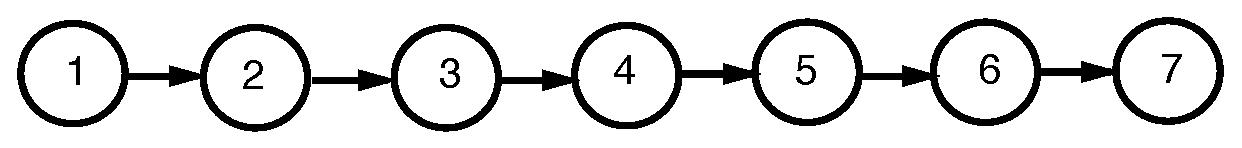
\includegraphics[width=11cm, height=1cm]{images/network_diagram.eps}
				\caption{Сетевой график выполнения работ\label{img:network_diagram}}
			\end{figure}

			Обозначение выполняемых работ:
			\begin{itemize}
				\item 1 --- 2 - формирование требований к ИС (2 дня);
				\item 2 --- 3 - разработка задач ИС и ТЗ (5 дней);
				\item 3 --- 4 - технический проект (14 дней);
				\item 4 --- 5 - рабочая документация, настройка системы и знакомство её с пользователями (4 дня);
				\item 5 --- 6 - ввод в действие (2 дня);
				\item 6 --- 7 - сопровождение АС (15 дней).
			\end{itemize}

			Длительность критического пути составляет $\text{Т}_{\text{кр}}$  = 42 дня.

			\indent Каждый из специалистов задействован на проекте следующее число дней:
			\begin{itemize}
				\item прикладной математик --- 7 дней;
				\item проектировщик --- 13 дней;
				\item разработчик (backend) --- 19 дней;
				\item разработчик (frontend) --- 6 дней;
				\item тестировщик --- 17 дней.
			\end{itemize}

			Затраты по заработной плате рассчитываются следующим образом:
			\begin{equation}\label{eq:salary}
				\text{З} = \text{З}_{\text{зп}} + \text{СВ}
			\end{equation}
				\begin{ESKDexplanation}
				\item[где ]$\text{З}_{\text{зп}}$ --- заработная плата задействованных специалистов, руб.;
				\item $\text{СВ}$ --- страховые взносы во внебюджетные фонды, руб..
			\end{ESKDexplanation}

			\begin{equation}\label{eq:salary_specialist}
				\text{З}_{\text{зп}} = \sum_{i=1}^{n} \frac{ \text{О}_i }{ \text{Д} } * t_i ,		
			\end{equation}
			\begin{ESKDexplanation}
				\item[где ] n --- количество задействованных специалистов, чел.;
				\item $\text{О}_i$ --- оклад i-го специалиста, руб.;
				\item $\text{Д}$ --- количество рабочих дней в месяце, дни;
				\item $t_i$ --- время участия специалиста в проекте (дни), определяется в соответствии с разработанным сетевым планом проектных работ.
			\end{ESKDexplanation}

			Отчисления в Фонд оплаты труда составляют 30\%:
			\begin{equation}\label{eq:royalty}
				\text{СВ} = \text{З}_{\text{зп}} * 0,3
			\end{equation}

			Учитывая разработанные сетевой график и квалификационный план выполнения проектных работ, затраты на заработную плату задействованных специалистов составляют:
			$$\text{З}_{\text{зп}} = 162\,500,00 \text{ руб.}$$

			С полученной суммы в фонд оплаты труда производятся отчисления в размере:
			$$\text{СВ} = 162\,500,00 * 0,3 = 48\,750,00 \text{ руб.}$$

			В итоге затраты по заработной плате состовляют:
			$$\text{З} = 162\,500,00 + 48\,750,00 = 211\,250,00 \text{ руб.}$$

			Основными расходными материалами и нематериальными активами, задействованными при разработке ИС, являются электроэнергия, необходимая для работы компьютеров, и широкополосный доступ в Интернет.

			В процессе разработки  системы задействовано семь компьютеров: по одному на каждого из участиков проекта, один компьютер для разворачивания ИС и один - для запуска СУБД. Средняя номинальная мощность каждого компьютера составляет 100 Вт/ч.

			Затраты на расходные материалы вычисляются по следующей формуле:
			\begin{equation}\label{eq:consumables}
				\text{М} = \text{И} + \text{Э},
			\end{equation}
			\begin{ESKDexplanation}
				\item[где ]$\text{М}$ --- стоимость затраченных расходных материалов, руб.;
				\item $\text{И}$ ---  стоимость услуг интернета, руб.;
				\item $\text{Э}$ ---  стоимость электроэнергии, руб.
			\end{ESKDexplanation}

			Стоимость электроэнергии рассчитывается по следующей формуле:
			\begin{equation}\label{eq:cost_power}
				\text{Э} = \text{Р} * \text{Ц} * \text{Т},
			\end{equation}
			\begin{ESKDexplanation}
				\item[где ]$\text{Р}$ ---  мощность компьютера, кВ;
				\item $\text{Ц}$ ---  цена электроэнергии за кВ.ч, руб..		
			\end{ESKDexplanation}

			Результаты расчета затрат на расходные материалы сведены в таблицу \ref{tab:consumables}.

			\begin{table}[h]
				\small
				\centering
				\caption{Затраты на расходные материалы}
				\label{tab:consumables}								
				\begin{tabular}{|l|l|l|l|}				
				\hline
					\multicolumn{1}{|c|}{Наименование} 										&
					\multicolumn{1}{ c|}{Цена, руб.} 										&
					\multicolumn{1}{ c|}{Количество, ед.} 									&		
					\multicolumn{1}{ c|}{Стоимость, руб (с учетом НДС)} 					\\ \hline
					\multicolumn{1}{|c|}{Электроэнергия} 															&
					\multicolumn{1}{ c|}{3,20}	 																& 
					\multicolumn{1}{ c|}{7 * 0,1 * 12 * 42} 														&
					\multicolumn{1}{ c|}{352,80} 																	\\ \hline
					\multicolumn{1}{|c|}{Интернет} 																&
					\multicolumn{1}{ c|}{4 000,00}																&
					\multicolumn{1}{ c|}{1}																		&
					\multicolumn{1}{ c|}{4 000,00} 																\\ \hline
				\end{tabular}
			\end{table}					

			Амортизация оборудования вычисляется по следующей формуле:
			\begin{equation}\label{eq:amortization}
				A = A_1 + A_2,
			\end{equation}
			\begin{ESKDexplanation}
				\item[где ]$A$ --- общая амортизация, руб.;
				\item $A_1$ --- амортизация ЭВМ, руб.;
				\item $A_2$ --- амортизация сетевого оборудования, руб..
			\end{ESKDexplanation}

			В таблице \ref{tab:norm_amortization} приведены расчеты норм амортизации оборудования, а в таблицу \ref{tab:cost_amortization} сведены затраты на амортизацию оборудования и нематериальных активов, используемых в процессе разработки системы.

			\begin{table}[h]
				\small
				\centering
				\caption{Расчеты норм амортизации оборудования и  программного обеспечения}
				\label{tab:norm_amortization}								
				\begin{tabular}{|l|l|l|l|l|}				
				\hline
					\multicolumn{1}{|c|}{Наименование} 										&
					\multicolumn{1}{ c|}{Стоимость, руб.} 									&
					\multicolumn{1}{ p{3cm}|}{\centering Срок эксплуатации, лет} 			&		
					\multicolumn{1}{ p{3cm}|}{\centering Норма амортизации, руб./мес.} 		&	
					\multicolumn{1}{ p{3cm}|}{\centering Норма амортизации, руб./день} 		\\ \hline
					\multicolumn{1}{|p{3cm}|}{Компьютер} 																&
					\multicolumn{1}{ c|}{70 000,00} 																&
					\multicolumn{1}{ c|}{5}																	&
					\multicolumn{1}{ c|}{1170,00}																	&
					\multicolumn{1}{ c|}{53,00} 																	\\ \hline
					\multicolumn{1}{|p{3cm}|}{Роутеры} 																& 
					\multicolumn{1}{ c|}{5 000,00} 																& 
					\multicolumn{1}{ c|}{5} 																		& 
					\multicolumn{1}{ c|}{83,00} 																	& 
					\multicolumn{1}{ c|}{3,78} 																	\\ \hline
				\end{tabular}
			\end{table}

			\begin{table}[h]
				\small
				\centering
				\caption{Расчет амортизации оборудования и нематериальных активов}
				\label{tab:cost_amortization}								
				\begin{tabular}{|l|l|l|l|l|}				
				\hline
					\multicolumn{1}{|p{3cm}|}{\centeringНаименование} 						&
					\multicolumn{1}{ p{2cm}|}{\centeringКол-во, шт.}						&
					\multicolumn{1}{ p{4cm}|}{\centeringНорма амортизации, руб/день} 		&		
					\multicolumn{1}{ p{3cm}|}{\centeringДлительность, дни} 					&	
					\multicolumn{1}{ p{3cm}|}{\centeringСтоимость, руб.} 					\\ \hline
					\multicolumn{1}{|p{3cm}|}{Компьютер} 																&
					\multicolumn{1}{ c|}{7} 																		& 
					\multicolumn{1}{ c|}{371,00}																	&
					\multicolumn{1}{ c|}{42} 																		& 
					\multicolumn{1}{ c|}{15\,582,00} 																\\ \hline
					\multicolumn{1}{|p{3cm}|}{Роутеры}																& 
					\multicolumn{1}{ c|}{3} 																		& 
					\multicolumn{1}{ c|}{11,34} 																	& 
					\multicolumn{1}{ c|}{42} 																		& 
					\multicolumn{1}{ c|}{476,28} 																	\\ \hline
				\end{tabular}
			\end{table}					

			Исходя из полученных расчётов, стоимость разработки ИС состовялет:
			$$\text{С}_{\text{ис}} = 211\,250,00 + 352,80 + 4\,000,00 +  15\,582,00 + 476,28 = 231\,661,08 \text{ руб.}$$			
		
		\subsubsection{Расчет стоимости выполнения процесса до автоматизации}

			До внедрения ИС процесс проверки работы на плагиат состоит из следующих процессов:
			\begin{itemize}
				\item загрузка работы студента на локальную машину преподавателя;
				\item нахождение работ в системе Moodle для сравнения;
				\item ручная сверка новой работы с другими работами.
			\end{itemize}

			Для расчётов общей стоимости выполнения процесса необходимо расчитать стоимость каждой операции процесса. Стоимость операции рассчитывается как сумма затрат на заработную плату сотрудникам, на амортизацию оброрудования и на расходные материалы:
			\begin{equation}\label{eq:cost_before_automation}
				\text{С}_{\text{до}} = \sum_{i=1}^{n} \text{З}_{Oi} + \sum_{i=1}^{n} \text{М}_{Oi} + \sum_{i=1}^{n} \text{А}_{Oi} ,
			\end{equation}
			\begin{ESKDexplanation}
				\item[где ]$n$ – количество  операций в процессе, штук;
				\item $\text{З}_{Oi}$ --- заработная плата сотрудника при выполнении i-ой операции, руб.;
				\item $\text{М}_{Oi}$ --- затраты на расходные материалы, необходимые при выполнении i-ой операции, руб.;
				\item $\text{А}_{Oi}$ --- амортизация оборудования и нематериальных активов для i-ой  операции, руб..
			\end{ESKDexplanation}	
			
			При выполнении автоматизируемого процесса, как до, так и после автоматизации, затраты на расходные материалы отсутствуют в связи с тем, что все операции производятся исключительно на компьютере пользователя.


			В таблице \ref{tab:salary_before_automation} представлен расчёт затрат на заработную плтату сотрудникам.

			\begin{table}[h]
				\small
				\centering
				\caption{Расчет затрат на заработную плату сотрудникам, выполняющим процесс до автоматизации}
				\label{tab:salary_before_automation}								
				\begin{tabular}{|l|l|l|l|l|}				
				\hline
					\multicolumn{1}{|p{4cm}|}{\centering Операция} 							&
					\multicolumn{1}{ p{3cm}|}{\centering Время выполнения операции, час.} 	&
					\multicolumn{1}{ p{3cm}|}{\centering Зарплтата, руб./час.} 				&		
					\multicolumn{1}{ p{3cm}|}{\centering Количество сотрудников, чел.} 		&	
					\multicolumn{1}{ p{2cm}|}{\centering Затраты, руб.} 					\\ \hline
					\multicolumn{1}{|p{4cm}|}{Загрузка работы студента на локальную машину преподавателя}				& 
					\multicolumn{1}{ c|}{0,10}																	& 
					\multicolumn{1}{ c|}{170,45}																	& 
					\multicolumn{1}{ c|}{1} 																		& 
					\multicolumn{1}{ c|}{22,15}																	\\ \hline
					\multicolumn{1}{|p{4cm}|}{Нахождение работ в системе Moodle для сравнения}		 				& 
					\multicolumn{1}{ c|}{0,20} 																	& 
					\multicolumn{1}{ c|}{170,45} 																	& 
					\multicolumn{1}{ c|}{1}																		& 
					\multicolumn{1}{ c|}{44,31}																	\\ \hline
					\multicolumn{1}{|p{4cm}|}{Ручная сверка новой работы с другими работами}						& 
					\multicolumn{1}{ c|}{3,5}																	& 
					\multicolumn{1}{ c|}{170,45}																	& 
					\multicolumn{1}{ c|}{1}																		&
					\multicolumn{1}{ c|}{775,55} 																	\\ \hline
					Итого & & & & \multicolumn{1}{ c|}{842,01}													\\ \hline
				\end{tabular}
			\end{table}								

			Затарты на амотризацию компьютеров состовляют 123,32 руб.

			$$ \text{С}_{\text{до}} = 965,33 \text{ руб.}$$

		\subsubsection{Расчет стоимости выполнения процесса после автоматизации}

			После внедрения ИС процесс проверки работы на плагиат состоит из следующих процессов:
			\begin{itemize}
				\item просмотр результата проверки работы на плагиат;
				\item ручной запуск проверки на плагиат новой работы;
				\item обработка запроса системой проверки на плагиат;
				\item анализ результата проверки на плагиат.
			\end{itemize}

			Для расчётов общей стоимости выполнения процесса необходимо расчитать стоимость каждой операции процесса. Стоимость операции рассчитывается как сумма затрат на заработную плату сотрудникам и на амортизацию оброрудования:
			\begin{equation}\label{eq:cost_after_automation}
				\text{С}_{\text{после}} = \sum_{i=1}^{n} \text{З}_{Oi} + \sum_{i=1}^{n} \text{М}_{Oi} + \sum_{i=1}^{n} \text{А}_{Oi} ,
			\end{equation}
			\begin{ESKDexplanation}
				\item[где ]$n$ – количество  операций в процессе, штук;
				\item $\text{З}_{Oi}$ --- заработная плата сотрудника при выполнении i-ой операции, руб.;
				\item $\text{М}_{Oi}$ --- затраты на расходные материалы, необходимые при выполнении i-ой операции, руб.;
				\item $\text{А}_{Oi}$ --- амортизация оборудования и нематериальных активов для i-ой  операции, руб..
			\end{ESKDexplanation}

			В таблице \ref{tab:salary_after_automation} представлен расчёт затрат на заработную плтату сотрудникам.

			\begin{table}[h]
				\small
				\centering
				\caption{Расчет затрат на заработную плату сотрудникам, выполняющим процесс после автоматизации}
				\label{tab:salary_after_automation}								
				\begin{tabular}{|C{5cm}|C{2cm}|C{2cm}|C{2cm}|C{3cm}|}				
				\hline
					{Операция} 											&
					{Время выполнения операции, час.} 					&
					{Зарплтата, руб./час.} 								&		
					{Количество сотрудников, чел.} 						&	
					{Затраты, руб.} 									\\ \hline
					\multicolumn{1}{|p{5cm}|}{Просмотр результата проверки работы на плагиат} 							& 
					0,05 																	& 
					170,45 																	& 
					1 																		& 
					8,52 																	\\ \hline
					\multicolumn{1}{|p{5cm}|}{Ручной запуск проверки на плагиат новой работы} 							& 
					0,1 																	& 
					170,45 																	& 
					1 																		& 
					17,05 																	\\ \hline
					\multicolumn{1}{|p{5cm}|}{Анализ результата проверки на плагиат} 									& 
					0,2 																	& 
					170,45 																	& 
					1 																		& 
					34,09 																	\\ \hline 
					\multicolumn{1}{|p{5cm}|}{Итого} & & & & 59,66 													\\ \hline
				\end{tabular}
			\end{table}			

			Затарты на амотризацию компьютеров состовляют 178,73 руб.

		\newpage
		\subsubsection{Расчет экономического эффекта от внедрения подсистемы}
			Годовая экономия рассчитывается по формуле:
			\begin{equation}\label{eq:annual_performance}
				\text{Э} = (\text{С}_{\text{до}} - \text{С}_{\text{после}}) * 100,
			\end{equation}
			$$ \text{Э} = 78\,235,00 \text{руб.}$$

			Годовой экономический эффект рассчитывается по формуле:
			\begin{equation}\label{eq:annual_economic_effect}
				\text{Э}_{\text{г}} = \text{Э} - \text{Е}_{\text{н}} * \text{С}_{\text{ис}},				
			\end{equation}
			\begin{ESKDexplanation}
				\item[где ] Э --- годовая экономия, руб.;
				\item $\text{Е}_{\text{н}}$ --- нормативная эффективность капиталовложений (0,25);
				\item $\text{С}_{\text{ис}}$ --- стоимость разработки подсистемы, руб..
			\end{ESKDexplanation}
			$$\text{Э}_{\text{г}} = 158\,235,00 - 0,25 * 231\,661,08 = 90\,319,73 \text{ руб.}$$

			Исходя из полученных результатов расчета годового экономического эффекта, можно рассчитать коэффициент экономической эффективности:
			\begin{equation}\label{eq:cost_effectiveness_ratio}
				\text{Е} = \text{Э}_{\text{г}} / \text{С}_{\text{ис}},				
			\end{equation}
			\begin{ESKDexplanation}
				\item[где ]$\text{Э}_{\text{г}}$ --- годовой экономический эффект;					
				\item $\text{С}_{\text{ис}}$ --- стоимость разработки подсистемы, руб..
			\end{ESKDexplanation}
			$$\text{Е} = 90\,319,73 / 231\,661,08 = 0,39.$$

			Срок окупаемости данного проекта можно рассчитать по формуле:
			\begin{equation}\label{eq:payback_period}
				\text{Т} = 1 / \text{Е}				
			\end{equation}

			Таким образом, срок окупаемости данного проекта составляет:
			$$\text{Т} = 1 / 0,39 = 2,6 \text{ года}.$$

			Рассчитанные показатели свидетельствуют об экономической эффективности проектируемой ИС <<Шерлок>>.

	\subsection{Инструкция по эксплуатации информационной системы <<Шерлок>>}

		При работе с ИС <<Шерлок>> принимает участие несколько типов пользователей:
		\begin{itemize}
			\item администратор - устанавливает и настраивает работу серверной части ИС (<<backend>>);
			\item сотрудник учебного заведения - взаимодействует с графическим интерфейсом ИС (<<frontend>>);
			\item стороние разработчики - создают сторонние сервисы, которые взаимодействуют с <<backend>>-частью ИС.			
		\end{itemize}

		Далее приведены инструкции для каждого из типов пользователей.

		\subsubsection{Инструкция для администратора}

			ИС <<Шерлок>> распространяется в виде одного jar-файла, который запускается и выполняется на платформе Java, и конфигурационного файла app.config, в котором хранится информация о настройках ИС.

			Перед запуском ИС необходимо установить и настроить следующее ПО на двух рабочих станциях:
			\begin{itemize}
				\item первая рабочая станция - платформа Java (JRE) \cite{web:java}. После установки первая рабочая станция готова к запуску ИС <<Шерлок>>;
				\item вторая рабочая станция - СУБД MongoDB \cite{web:mongodb}. После установки СУБД необходимо произвести её начальную настройку: указать, с каких IP адресов будет доступна база; создать базу данных и пользователя, который имеет доступ к этой БД.
			\end{itemize}

			Перед запуском ИС <<Шерлок>> необходимо настроить систему для работы с БД. Для этого в файле app.properties указывается строка следующего вида:
			$$mongodb://{login}:{password}@{host}/{db},$$
			\begin{ESKDexplanation}
				\item[где ] $\text{login}$ --- логин пользователя для доступа к БД;
				\item $\text{password}$ --- пароль пользователя для доступа к БД;
				\item $\text{host}$ --- адрес машины, на которой работает СУБД;
				\item $\text{db}$ --- название ранее созданой БД.				
			\end{ESKDexplanation}

			Более подробные сведения о подключении к БД можно узнать из документации к Spring Framework \cite{web:mongodb_manual}. После этого система готова к запуску.

			Для запуска ИС на ОС семейства Unix необходимо выполнить следующие действия в консоли:
			\begin{itemize}
				\item перейти в директорию, где располагается файл ИС (sherlock.jar);
				\item запустить ИС следующей командой: $java -jar\ ./sherlock.jar$.
			\end{itemize}

			После этого система запущена и готова к работе.

			Для интеграции Moodle с ИС <<Шерлок>> необходимо произвести установку плагина в соответсвии с инструкцией, распологающейся на оффициальном сайте Moodle.

		\subsubsection{Инструкция для сотрудника учебного заведения}

			Проверка новых студенческих работ на плагиат происходит при загрузке работы студента в Moodle, поэтому при проверке сотрудником работы, ему уже будет доступен результат проверки в виде процентного значения совпадения с другим работами от 0\% до 100\% и ссылка на работу, которая наиболее схожа с проверяемой.

		\subsubsection{Инструкция для разработчиков}

			Несмотря на то, что в рамках данной работы ИС <<Шерлок>> разрабатывается для решения задач в учебной среде, применение ИС не ограничивается только этой средой, а может применятся и в других сферах деятельности человека.

			При проектировании ИС было учтено, что взаимодействие с ней может происходить из совершенно различных систем в плане технической реализации. По этому в качестве реализации интерфейса к ИС (API) был выбран подход REST, который позволяет взаимодействовать с системой посредством обычных HTTP-запросов.

			В таблице \ref{tab:api_method} представлены основные методы взаимодействия с ИС <<Шерлок>>, которые доступны в текущей версии ИС:

			\begin{table}[h]
				\small
				\centering
				\caption{Описание HTTP-методов для взаимодействия с системой}
				\label{tab:api_method}								
				\begin{tabular}{|l|l|p{5cm}|p{5cm}|}				
				\hline
					\multicolumn{1}{|c|}{URL} 												&
					\multicolumn{1}{ c|}{Метод HTTP} 										&
					\multicolumn{1}{ c|}{Описание} 											&		
					\multicolumn{1}{ c|}{Параметры} 										\\ \hline
					/similarity/sync 														& 
					POST 																	& 
					запрос на синхронную проверку работы на плагиат 						&
					sourceText - исходный код проверяемой программы 						\\ \hline
					/similarity/async 														& 
					POST 																	& 
					запрос на асинхронную проверку работы на плагиат. В ответ система генерирует уникальный идетификатор, по которому пользователь в последствии может получить результат проверки &
					sourceText - исходный код проверяемой программы 						\\ \hline
					/similarity/result/ 													& 
					GET 																	& 
					запрос на получение результата проверки на плагиат	 					& 
					uuid - уникальный идентификатор, полученный пользователем при асинхронном запросе на проверку																 \\ \hline
					/user/create 															& 
					POST 																	&
					запрос на создание новой учётной записи пользователя в системе			&
					username - логин нового пользователя; password - пароль нового пользователя \\ \hline
				\end{tabular}
			\end{table}